\documentclass[11pt]{article}
\usepackage{icmlko}
\begin{document}

\title{표지는 봉우리가 있다 --- 판을 통과한 변경을 처음으로 물렸다}
\author{월드모델 실험실}
\date{노트 420 · 2026년 8월 2일}
\maketitle

\begin{abstract}
노트 419가 다음 방향을 정했다 --- \emph{전이를 사는 것은 도메인 가르는 일을
떠맡는 표지다. grp 는 도메인당 값 하나뿐이니 더 주면 더 사나.} 두 번째
표지를 지었다: 웹툰 \texttt{daily\_pass} · 모바일 \texttt{advisory} ·
애니 \texttt{is\_original} · 세계애니 \texttt{source} · \textbf{만화
\texttt{format}} · 게임 \texttt{n\_platform} · 펀딩 \texttt{adult\_only} ·
도서 \texttt{book\_format}. 전부 기획 시점 값이고(\texttt{status} ·
\texttt{finished} 같은 사후 값은 뺐다), \textbf{여덟 도메인}을 덮는다 ---
grp 가 못 덮는 \textbf{만화까지}.

\begin{center}
\begin{tabular}{lr}
\hline
grp2 를 넣으면 & \\
\hline
\textbf{판} (짝 12뽑기) & $\mathbf{+0.0035 \pm 0.0024 \cdot 11/12}$ \\
\textbf{KR 만화 전이} & $+0.1946 \to \mathbf{+0.0806}$ \\
\quad 같은 유보 행 짝 되뽑기 차 & $+0.1140$, 95\% $[+0.0674, +0.1589]$, $800/800$ \\
\hline
\end{tabular}
\end{center}

\textbf{판은 조건 ① 을 넘는다}(부호 $11/12$). 그런데 \textbf{전이를 확실히
잃는다.} 사전 등록의 실패 조건이 그대로 걸렸다 --- \emph{전이가 안 오르면
``더 갈라 주면 더 산다''가 틀린 것이고, grp 의 이득은 한 번만 나는 것이지
양에 비례하지 않는다.}

\textbf{안 넣었다.} 규약을 통과한 변경을 물린 것은 이번이 처음이다.
\end{abstract}

\section{표지의 봉우리}

표지 개수로 놓고 보면 모양이 분명하다.

\begin{center}
\begin{tabular}{lr}
\hline
도메인 표지 & KR 만화 전이 \\
\hline
0 개 (grp 없음) & $-0.0822$ \\
\textbf{1 개 (grp)} & $\mathbf{+0.2128}$ \\
2 개 (grp $+$ grp2) & $+0.0806$ \\
\hline
\end{tabular}
\end{center}

\textbf{하나는 사고 둘째는 되판다.} 읽기: 첫 표지는 나무가 공유 축으로
도메인을 가르던 일을 대신 맡아 축을 풀어 준다(노트 413·417). 둘째부터는
\textbf{학습 도메인 집합을 더 잘게 깎는 데} 쓰이고, 그렇게 깎을수록 모형이
\emph{그 열한 개}에 맞춰진다 --- 안 본 도메인은 그만큼 멀어진다.

노트 396이 알파 · $\tau$ · 깊이를 두고 적은 말이 여기에도 맞다 ---
\textbf{봉우리가 있는 손잡이는 안쪽에서 고르면 빗나간다.} 다만 이번 봉우리는
판이 아니라 \textbf{전이} 위에 있고, 판만 보면 봉우리가 안 보인다.

\section{규약을 하나 더한다}

지금까지 규약은 판만 말했다 --- 조건 ① 을 넘으면 넣는다. 노트 399부터 407까지
``판은 지키라 하고 목표는 빼라 한다''는 긴장을 그때그때 사람이 판정했고,
노트 417에서 처음으로 둘이 일치했다.

이번은 반대 방향이다: \textbf{판이 넣으라 하고 목표가 물리라 한다.} 그래서
적는다.

\begin{center}
\textbf{전이를 확실히 잃는 변경은 판이 통과해도 안 넣는다.}\\
(``확실히'' $=$ 같은 유보 행 짝 되뽑기 구간이 0 을 안 물 때)
\end{center}

값은 판 $+0.0035$ 다. 전이 $-0.1140$ 과 견주면 싸다.

\section{남은 것}

\begin{tabular}{lp{7.0cm}}
\hline
grp2 는 지어 두고 안 쓴다 & \texttt{lab/grpaxes.py} 의 \texttt{build2}.
주석에 판정을 적어 뒀다 --- 그냥 꽂으면 판만 보고 목표를 잃는다 \\
표지 하나를 더 좋게 & 개수가 아니라 \textbf{질}이라면, grp 의 여덟 field 를
바꿔 가며 재는 것이 다음 시험이다 \\
웹툰 & grp2 에서 처음으로 크게 벌었다($+0.0166 \cdot 12/12$). 여섯 번
설명에 실패한 그 도메인이 무엇에 반응하는지 실마리일 수 있다 \\
\hline
\end{tabular}

\begin{figure}[h]
\centering
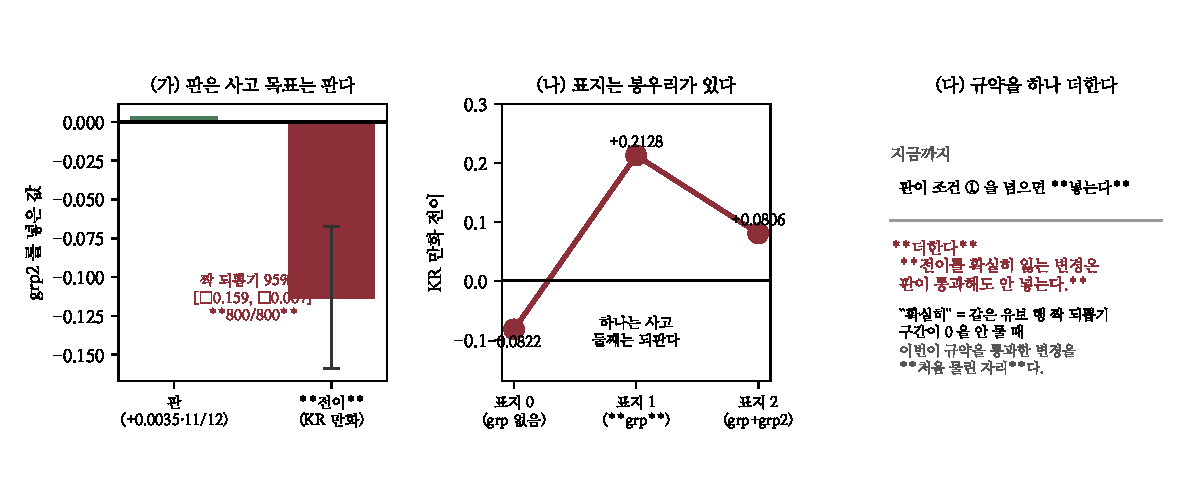
\includegraphics[width=\textwidth]{figs/fig420.pdf}
\caption{(가) 판은 사고 목표는 판다. (나) 표지 개수와 전이 --- 봉우리가 1 에
있다. (다) 새 규약.}
\end{figure}

\end{document}
